% !TeX program = xelatex
\documentclass[a4paper,10pt]{article}

% ============================================================================
% ១. កញ្ចប់បណ្ណាល័យ និងការកំណត់ទំព័រ (Packages & Page Setup — តាមគំរូ ls_plan.tex)
% ============================================================================
\usepackage[a4paper, left=0.95cm, right=0.95cm, top=0.85cm, bottom=0.92cm, footskip=0.52cm]{geometry}
\usepackage{amsmath}
\usepackage{unicode-math}
\usepackage{fontspec}
\usepackage{longtable, array, multirow, colortbl}
\usepackage[table]{xcolor}
\usepackage{enumitem}
\usepackage{pifont}
\usepackage{fancyhdr}
\usepackage{tikz}
\usetikzlibrary{calc, arrows.meta, decorations.pathreplacing, patterns, positioning, babel}

\makeatletter
\let\@expl@@@mark@update@singlecol@structures@@\relax
\makeatother

% --- ប្រព័ន្ធស្វែងរកទីតាំងពុម្ពអក្សរស្វ័យប្រវត្តិ (Windows Local + Cloud Repo fonts/) ---
\providecommand{\NGSFindFonts}{%
  \IfFileExists{C:/Windows/Fonts/cambria.ttc}{%
    \def\NGSSysPath{C:/Windows/Fonts/}%
    \def\NGSUserPath{C:/Users/KIT/AppData/Local/Microsoft/Windows/Fonts/}%
  }{%
    \IfFileExists{./fonts/KhmerOSsiemreap.ttf}{\def\NGSSysPath{./fonts/}\def\NGSUserPath{./fonts/}}{%
    \IfFileExists{../fonts/KhmerOSsiemreap.ttf}{\def\NGSSysPath{../fonts/}\def\NGSUserPath{../fonts/}}{%
    \IfFileExists{../../fonts/KhmerOSsiemreap.ttf}{\def\NGSSysPath{../../fonts/}\def\NGSUserPath{../../fonts/}}{%
    \IfFileExists{../../../fonts/KhmerOSsiemreap.ttf}{\def\NGSSysPath{../../../fonts/}\def\NGSUserPath{../../../fonts/}}{%
    \IfFileExists{../../../../fonts/KhmerOSsiemreap.ttf}{\def\NGSSysPath{../../../../fonts/}\def\NGSUserPath{../../../../fonts/}}{%
    \IfFileExists{../../../../../fonts/KhmerOSsiemreap.ttf}{\def\NGSSysPath{../../../../../fonts/}\def\NGSUserPath{../../../../../fonts/}}{%
    \IfFileExists{../../../../../../fonts/KhmerOSsiemreap.ttf}{\def\NGSSysPath{../../../../../../fonts/}\def\NGSUserPath{../../../../../../fonts/}}{%
      \def\NGSSysPath{../../../../../../../fonts/}\def\NGSUserPath{../../../../../../../fonts/}%
    }}}}}}}%
  }%
}
\NGSFindFonts

% ============================================================================
% ២. កំណត់ពុម្ពអក្សរ (Fonts — តាមគំរូ ls_plan.tex)
% ============================================================================
\setmathfont[Path={\NGSSysPath}, FontIndex=1, Scale=1.02]{cambria.ttc}
\defaultfontfeatures{Ligatures=TeX}

\setmainfont[
  Path={\NGSUserPath},
  Extension=.ttf,
  Script=Khmer,
  BoldFont={KhmerOSsiemreap},
  BoldFeatures={FakeBold=1.8},
  ItalicFont={KhmerOSsiemreap},
  ItalicFeatures={FakeSlant=0.25},
  BoldItalicFont={KhmerOSsiemreap},
  BoldItalicFeatures={FakeBold=1.8, FakeSlant=0.25}
]{KhmerOSsiemreap}

\newfontfamily\muol[Path={\NGSUserPath}, Extension=.ttf, Script=Khmer]{KhmerOSmuollight}
\newfontfamily\Tacteing[Path={\NGSUserPath}, Extension=.TTF]{TACTENG}
\newfontfamily\TimesEn[Path={\NGSSysPath}, Extension=.ttf, BoldFont={timesbd}, ItalicFont={timesi}, BoldItalicFont={timesbi}]{times}
\newfontfamily\CalibriFont[Path={\NGSSysPath}, Extension=.ttf]{calibri}
\newfontfamily\CourierCirc[Path={\NGSSysPath}, Extension=.ttf]{cour}

\XeTeXlinebreaklocale "km"
\XeTeXlinebreakskip = 0pt plus 1pt minus 0.1pt

% ============================================================================
% ៣. ពណ៌ និងការតុបតែង (Colors & Styles)
% ============================================================================
\definecolor{stepbg}{HTML}{D9D9D9}
\definecolor{headgray}{HTML}{E6E6E6}
\definecolor{emphred}{HTML}{C00000}

\pagestyle{fancy}
\fancyhf{}
\renewcommand{\headrulewidth}{0pt}
\fancyfoot[R]{\CalibriFont\fontsize{9pt}{11pt}\selectfont\thepage}

\setlength{\parindent}{0pt}
\setlength{\parskip}{0pt}
\setlength{\tabcolsep}{4.5pt}
\setlength{\LTpre}{2pt}
\setlength{\LTpost}{2pt}

\newcolumntype{L}[1]{>{\raggedright\arraybackslash}p{#1}}
\newcolumntype{C}[1]{>{\centering\arraybackslash}p{#1}}

% ============================================================================
% ៤. ពាក្យបញ្ជាជំនួយ (Helper Macros)
% ============================================================================
\newcommand{\en}[1]{{\TimesEn #1}}
\newcommand{\enbf}[1]{{\TimesEn\bfseries #1}}
\newcommand{\khmflourish}{{\Tacteing\fontsize{15pt}{15pt}\selectfont 3}}
\newcommand{\wcirc}{{\CourierCirc\fontsize{9.5pt}{11pt}\selectfont o}}
\newcommand{\ditem}{{\fontsize{7.5pt}{10pt}\selectfont\ding{117}}\ }
\newcommand{\fiveE}[1]{\textcolor{emphred}{\CalibriFont\bfseries #1}}
\newcommand{\redsub}[1]{\textcolor{emphred}{#1}}
\newcommand{\timenote}[1]{\textcolor{emphred}{\textit{#1}}}
\newcommand{\stepheader}[1]{\multicolumn{3}{|c|}{\cellcolor{stepbg}\muol #1} \\ \hline}
\newcommand{\cfig}[1]{{\centering\vspace{3pt}#1\vspace{3pt}\par}}
\newcommand{\cnum}[1]{\mbox{\fontsize{10.5pt}{12pt}\selectfont\ding{\numexpr181+#1\relax}}}
\newcommand{\unit}[1]{\,\text{\en{#1}}}
\newcommand{\riel}{\,\text{៛}}
\newcommand{\graybox}[1]{\colorbox{headgray}{\strut #1}}

% ============================================================================
% ៥. រូបភាព TikZ ស-ខ្មៅ សម្រាប់បង្រៀនលើក្ដារខៀន និងសន្លឹកកិច្ចការ (B&W Diagrams)
% ============================================================================

% ១. E1 Engage: បេសកកម្មស្លាកកញ្ចប់ក្រដាសរ៉ាម 80 g/m^2
\newcommand{\figEngageMEASFourTwo}{%
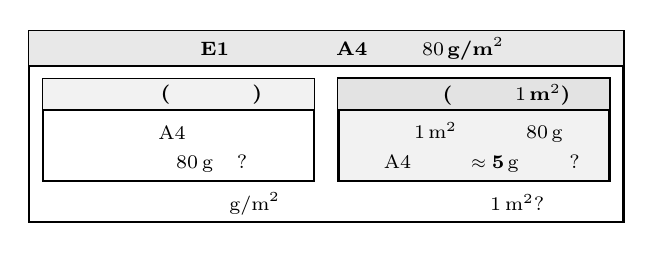
\begin{tikzpicture}[x=1cm, y=1cm, every node/.style={font=\scriptsize, text=black}]
  \draw[black, line width=0.9pt] (0,0) rectangle (7.55,2.42);
  \fill[gray!18] (0,1.98) rectangle (7.55,2.42);
  \draw[black, line width=0.6pt] (0,1.98) -- (7.55,1.98);
  \node at (3.775,2.20) {\textbf{បេសកកម្ម \en{E1}៖ ស្លាកក្រដាសរ៉ាម $\unit{A4}$ សរសេរថា $80\unit{g/m}^2$}};

  % Left: Student A (Misconception)
  \draw[black, line width=0.8pt] (0.18,0.52) rectangle (3.62,1.82);
  \fill[gray!10] (0.18,1.42) rectangle (3.62,1.82);
  \draw[black, line width=0.5pt] (0.18,1.42) -- (3.62,1.42);
  \node at (1.90,1.62) {\textbf{មតិសិស្ស ក (គិតលើ ១ សន្លឹក)}};
  \node at (1.90,1.14) {ក្រដាស $\unit{A4}$ មួយសន្លឹក};
  \node at (1.90,0.74) {មានម៉ាសស្មើ $80\unit{g}$ គត់?};

  % Right: Student B (Unit-area truth)
  \draw[black, line width=0.95pt, fill=gray!10] (3.93,0.52) rectangle (7.37,1.82);
  \fill[gray!22] (3.93,1.42) rectangle (7.37,1.82);
  \draw[black, line width=0.55pt] (3.93,1.42) -- (7.37,1.42);
  \node at (5.65,1.62) {\textbf{មតិសិស្ស ខ (ធៀបនឹងផ្ទៃ $1\unit{m}^2$)}};
  \node at (5.65,1.14) {ផ្ទៃ $1\unit{m}^2$ ទើបមានម៉ាស $80\unit{g}$};
  \node at (5.65,0.74) {ឯ $\unit{A4}$ ១ សន្លឹក $\approx \mathbf{5\unit{g}}$ ប៉ុណ្ណោះ?};

  \node at (3.775,0.23) {\textbf{សំណួរគន្លឹះ៖} តើខ្នាត $\unit{g/m}^2$ ប្រាប់ម៉ាសក្នុង ១ សន្លឹក ឬក្នុងផ្ទៃ $1\unit{m}^2$?};
\end{tikzpicture}}

% ២. E2 Explore: លំហាត់គំរូទី ១ (ទំ.៤៥ — ក្រដាសរ៉ាម ១ ដុំ 500 សន្លឹក, 210mm x 297mm, 80 g/m^2)
\newcommand{\figReamModelMEASFourTwo}{%
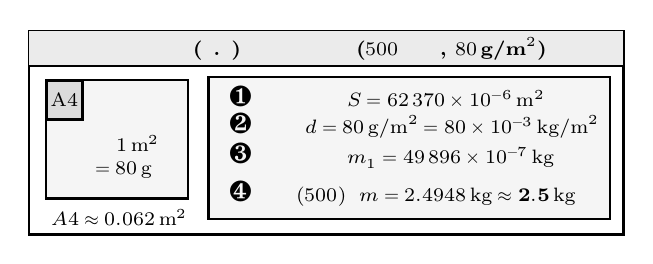
\begin{tikzpicture}[x=1cm, y=1cm, every node/.style={font=\scriptsize, text=black}]
  \draw[black, line width=0.9pt] (0,0) rectangle (7.55,2.58);
  \fill[gray!16] (0,2.14) rectangle (7.55,2.58);
  \draw[black, line width=0.6pt] (0,2.14) -- (7.55,2.14);
  \node at (3.775,2.36) {\textbf{លំហាត់គំរូទី ១ (ទំ.៤៥)៖ ក្រដាសរ៉ាម ១ ដុំ ($500$ សន្លឹក, $80\unit{g/m}^2$)}};

  % 1m x 1m vs A4 visual on left
  \draw[black, line width=0.85pt, fill=gray!8] (0.22,0.46) rectangle (2.02,1.96);
  \draw[black, line width=0.95pt, fill=gray!28] (0.22,1.46) rectangle (0.68,1.96);
  \node at (0.45,1.71) {\en{A4}};
  \node at (1.20,1.16) {ផ្ទៃ $1\unit{m}^2$};
  \node at (1.20,0.82) {$= 80\unit{g}$};
  \node at (1.15,0.22) {$\en{A4} \approx 0.062\unit{m}^2$};

  % Steps on right
  \draw[black, line width=0.8pt, fill=gray!8] (2.28,0.20) rectangle (7.38,2.00);
  \node[anchor=west] at (2.42,1.76) {\cnum{1} ផ្ទៃ ១ សន្លឹក៖ $S = 62\,370\times 10^{-6}\unit{m}^2$};
  \node[anchor=west] at (2.42,1.38) {\cnum{2} បំប្លែង $d = 80\unit{g/m}^2 = 80\times 10^{-3}\unit{kg/m}^2$};
  \node[anchor=west] at (2.42,1.00) {\cnum{3} ម៉ាស ១ សន្លឹក៖ $m_1 = 49\,896\times 10^{-7}\unit{kg}$};
  \node[anchor=west] at (2.42,0.52) {\cnum{4} ១ ដុំ ($500$)៖ $m = 2.4948\unit{kg} \approx \mathbf{2.5\unit{kg}}$};
\end{tikzpicture}}

% ៣. E3 Explain: រចនាសម្ព័ន្ធរូបមន្ត m = S x d និងការបូកចំនៀរខាត r%
\newcommand{\figFormulaTrimMEASFourTwo}{%
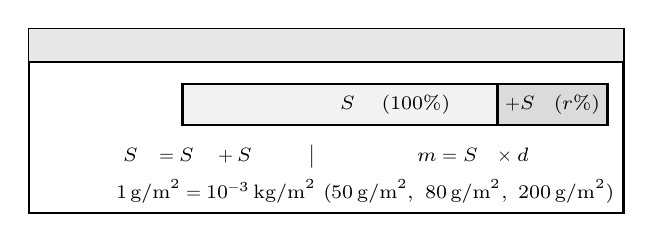
\begin{tikzpicture}[x=1cm, y=1cm, every node/.style={font=\scriptsize, text=black}]
  \draw[black, line width=0.9pt] (0,0) rectangle (7.55,2.34);
  \fill[gray!18] (0,1.92) rectangle (7.55,2.34);
  \draw[black, line width=0.6pt] (0,1.92) -- (7.55,1.92);
  \node at (3.775,2.13) {\textbf{រចនាសម្ព័ន្ធផ្ទៃក្រដាសសុទ្ធ និងចំនៀរខាតបង់ពេលកាត់}};

  % Bar diagram
  \node[anchor=west] at (0.18,1.38) {\textbf{ក្រដាសដើម៖}};
  \draw[black, line width=0.85pt, fill=gray!10] (1.95,1.12) rectangle (5.95,1.64);
  \node at (3.95,1.38) {ផ្ទៃក្រដាសរ៉ាមសុទ្ធ $S_{\text{សុទ្ធ}}$ ($100\%$)};
  \draw[black, line width=0.95pt, fill=gray!28] (5.95,1.12) rectangle (7.35,1.64);
  \node at (6.65,1.38) {$+S_{\text{ខាត}}$ ($r\%$)};

  \node at (3.775,0.72) {$S_{\text{សរុប}} = S_{\text{សុទ្ធ}} + S_{\text{ខាត}}$ \qquad $\big|$ \qquad ម៉ាសសរុប៖ $m = S_{\text{សរុប}} \times d$};
  \node at (3.775,0.28) {បំប្លែងខ្នាត៖ $1\unit{g/m}^2 = 10^{-3}\unit{kg/m}^2$ ($50\unit{g/m}^2, \ 80\unit{g/m}^2, \ 200\unit{g/m}^2$)};
\end{tikzpicture}}

% ៤. E4 Elaborate: លំហាត់គំរូទី ២ (ទំ.៤៥--៤៦ — កាត់ក្រដាស 70 g/m^2 ខាតចំនៀរ 4%)
\newcommand{\figTrimModelMEASFourTwo}{%
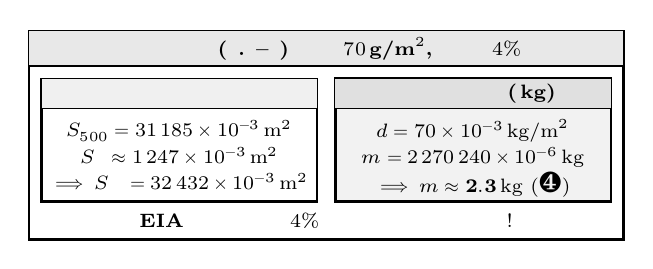
\begin{tikzpicture}[x=1cm, y=1cm, every node/.style={font=\scriptsize, text=black}]
  \draw[black, line width=0.9pt] (0,0) rectangle (7.55,2.64);
  \fill[gray!18] (0,2.20) rectangle (7.55,2.64);
  \draw[black, line width=0.6pt] (0,2.20) -- (7.55,2.20);
  \node at (3.775,2.42) {\textbf{លំហាត់គំរូទី ២ (ទំ.៤៥--៤៦)៖ ក្រដាស $70\unit{g/m}^2$, ខាតចំនៀរ $4\%$}};

  \draw[black, line width=0.8pt] (0.16,0.48) rectangle (3.66,2.04);
  \fill[gray!12] (0.16,1.66) rectangle (3.66,2.04);
  \draw[black, line width=0.55pt] (0.16,1.66) -- (3.66,1.66);
  \node at (1.91,1.85) {\textbf{ជំហានទី ១៖ ផ្ទៃក្រដាសសរុប}};
  \node at (1.91,1.38) {$S_{500} = 31\,185\times 10^{-3}\unit{m}^2$};
  \node at (1.91,1.04) {$S_{\text{ខាត}} \approx 1\,247\times 10^{-3}\unit{m}^2$};
  \node at (1.91,0.70) {$\implies S_{\text{សរុប}} = 32\,432\times 10^{-3}\unit{m}^2$};

  \draw[black, line width=0.95pt, fill=gray!10] (3.89,0.48) rectangle (7.39,2.04);
  \fill[gray!24] (3.89,1.66) rectangle (7.39,2.04);
  \draw[black, line width=0.6pt] (3.89,1.66) -- (7.39,1.66);
  \node at (5.64,1.85) {\textbf{ជំហានទី ២៖ ម៉ាសសរុប ($\unit{kg}$)}};
  \node at (5.64,1.38) {$d = 70\times 10^{-3}\unit{kg/m}^2$};
  \node at (5.64,1.04) {$m = 2\,270\,240\times 10^{-6}\unit{kg}$};
  \node at (5.64,0.70) {$\implies m \approx \mathbf{2.3\unit{kg}}$ (\cnum{4})};

  \node at (3.775,0.23) {\textbf{\en{EIA}៖} ត្រូវបូកចំនៀរខាត $4\%$ ព្រោះចំនៀរត្រូវកាត់ចោលពីក្រដាសដើម!};
\end{tikzpicture}}

% ៥. E5 Evaluate: ជម្រើសវិនិច្ឆ័យ A-D (ក្របសៀវភៅ 200 g/m^2, ផ្ទៃ 1 សន្លឹក = 0.5 m^2, ចំនួន 100 សន្លឹក)
\newcommand{\figExitMEASFourTwo}{%
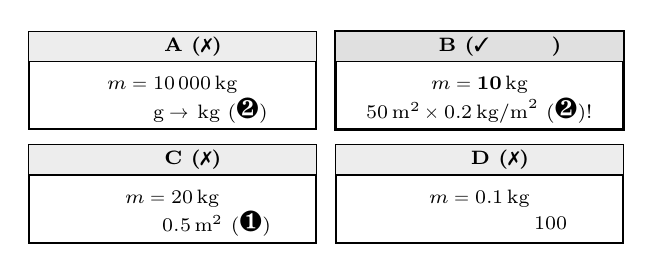
\begin{tikzpicture}[x=1cm, y=1cm, every node/.style={font=\scriptsize, text=black}]
  % Choice A
  \draw[black, line width=0.8pt] (0,1.44) rectangle (3.65,2.68);
  \fill[gray!14] (0,2.30) rectangle (3.65,2.68);
  \draw[black, line width=0.5pt] (0,2.30) -- (3.65,2.30);
  \node at (1.825,2.49) {\textbf{ជម្រើស \en{A} (\ding{55})}};
  \node at (1.825,2.00) {$m = 10\,000\unit{kg}$};
  \node at (1.825,1.68) {ភ្លេចបំប្លែង $\unit{g} \to \unit{kg}$ (\cnum{2})};

  % Choice B (Correct)
  \draw[black, line width=1.05pt] (3.90,1.44) rectangle (7.55,2.68);
  \fill[gray!24] (3.90,2.30) rectangle (7.55,2.68);
  \draw[black, line width=0.6pt] (3.90,2.30) -- (7.55,2.30);
  \node at (5.725,2.49) {\textbf{ជម្រើស \en{B} (\ding{51} ត្រឹមត្រូវ)}};
  \node at (5.725,2.00) {$m = \mathbf{10\unit{kg}}$};
  \node at (5.725,1.68) {$50\unit{m}^2 \times 0.2\unit{kg/m}^2$ (\cnum{2})!};

  % Choice C
  \draw[black, line width=0.8pt] (0,0) rectangle (3.65,1.24);
  \fill[gray!14] (0,0.86) rectangle (3.65,1.24);
  \draw[black, line width=0.5pt] (0,0.86) -- (3.65,0.86);
  \node at (1.825,1.05) {\textbf{ជម្រើស \en{C} (\ding{55})}};
  \node at (1.825,0.56) {$m = 20\unit{kg}$};
  \node at (1.825,0.24) {ភ្លេចគុណនឹងផ្ទៃ $0.5\unit{m}^2$ (\cnum{1})};

  % Choice D
  \draw[black, line width=0.8pt] (3.90,0) rectangle (7.55,1.24);
  \fill[gray!14] (3.90,0.86) rectangle (7.55,1.24);
  \draw[black, line width=0.5pt] (3.90,0.86) -- (7.55,0.86);
  \node at (5.725,1.05) {\textbf{ជម្រើស \en{D} (\ding{55})}};
  \node at (5.725,0.56) {$m = 0.1\unit{kg}$};
  \node at (5.725,0.24) {គណនាតែ ១ សន្លឹក ភ្លេចគុណ $100$};
\end{tikzpicture}}

\begin{document}
\fontsize{10pt}{15.2pt}\selectfont

% ============================================================================
% ក្បាលរដ្ឋបាល (Administrative Header — តាមគំរូ ls_plan.tex)
% ============================================================================
{\centering
  {\muol\fontsize{11pt}{16pt}\selectfont ព្រះរាជាណាចក្រកម្ពុជា\par}
  {\muol\fontsize{11pt}{16pt}\selectfont ជាតិ សាសនា ព្រះមហាក្សត្រ\par}
  \vspace{-3pt}{\khmflourish\par}
}

\vspace{1pt}
{\muol\fontsize{10pt}{15.5pt}\selectfont
មន្ទីរអប់រំ យុវជន និងកីឡា ខេត្តកំពង់ធំ\par
ការិយាល័យអប់រំ យុវជន និងកីឡា ស្រុកកំពង់ស្វាយ\par
អនុវិទ្យាល័យព្រះក្រសាំង\par}

\vspace{4pt}
{\centering{\muol\fontsize{11.5pt}{17pt}\selectfont កិច្ចតែងការបង្រៀន\par}}
\vspace{3pt}

% --- ព័ត៌មានទូទៅ ---
{\hspace*{2.8cm}\renewcommand{\arraystretch}{1.08}
\begin{tabular}{@{}l@{\hspace{0.35cm}}p{2.9cm}@{\hspace{0.15cm}}c@{\hspace{0.25cm}}l@{}}
  - & មុខវិជ្ជា & : & គណិតវិទ្យា ថ្នាក់ទី៨ (ពីជគណិត) \\
  - & ចំណងជើងមេរៀន & : & មេរៀនទី៤៖ រង្វាស់រង្វាល់ \\
  - & ចំណងជើងរង & : & ២. ម៉ាសធៀបនឹងផ្ទៃក្រឡា (ទំ.៤៤--៤៦, ៥០) \\
  - & រយៈពេល & : & ១ ម៉ោងសិក្សា (៥០ នាទី) \\
  - & បង្រៀនដោយ & : & ហុក ប៊ុនថែន \\
  - & កាលបរិច្ឆេទ & : & ថ្ងៃអង្គារ ទី១ ខែធ្នូ ឆ្នាំ២០២៦ \\
\end{tabular}\par}

\vspace{4pt}

% --- I. វត្ថុបំណង ---
{\muol\fontsize{10pt}{15.5pt}\selectfont \enbf{I.} វត្ថុបំណង\par}
\vspace{1pt}
{\renewcommand{\arraystretch}{1.10}
\begin{tabular}{@{}p{0.55cm}@{}p{2.35cm}@{\hspace{0.15cm}}c@{\hspace{0.25cm}}p{14.95cm}@{}}
  \hfill\wcirc\hspace{0.2cm} & វិជ្ជាសម្បទា & : & សិស្សប្រាប់អត្ថន័យនៃម៉ាសធៀបនឹងផ្ទៃក្រឡា ($d$ គិតជា $\unit{g/m}^2$ ឬ $\unit{kg/m}^2$ ដោយ $1\unit{g/m}^2 = 10^{-3}\unit{kg/m}^2$) រូបមន្ត $m = S\times d$ និងគោលការណ៍បូកភាគរយខាតបង់ចំនៀរក្រដាសបានត្រឹមត្រូវ ។ \\
  \hfill\wcirc\hspace{0.2cm} & បំណិនសម្បទា & : & សិស្សគណនាផ្ទៃក្រឡាក្រដាសជា $\unit{m}^2$ ម៉ាសក្រដាសរ៉ាម ១ ដុំ ($500$ សន្លឹក) និងម៉ាសក្រដាសសរុបពេលខាតចំនៀរ $4\%$ គិតជា $\unit{kg}$ តាមតារាងបណ្ដាក់ជំហានលើសន្លឹកកិច្ចការ (ទំ.៤៤--៤៦) បានត្រឹមត្រូវ ។ \\
  \hfill\wcirc\hspace{0.2cm} & ចរិយាសម្បទា & : & សិស្សមានទម្លាប់ពិនិត្យកម្រាស់ក្រដាស ($\unit{g/m}^2$) និងគណនាបរិមាណវត្ថុធាតុដើមក្នុងការផលិតសៀវភៅប្រកបដោយភាពសន្សំសំចៃនិងម៉ត់ចត់ ។ \\
\end{tabular}\par}

\vspace{3pt}

% --- II. សម្ភារៈឧបទេស ---
{\muol\fontsize{10pt}{15.5pt}\selectfont \enbf{II.} សម្ភារៈឧបទេស\par}
\vspace{1pt}
\hspace*{0.55cm}$\bullet$\ សៀវភៅសិក្សាគោលថ្នាក់ទី៨ (ទំ.៤៤--៤៦, ៥០) ក្ដារខៀន ដីស/ហ្វឺត បន្ទាត់ត្រង់ និង\textbf{សន្លឹកកិច្ចការសិស្សបំពេញចន្លោះ ស-ខ្មៅ} (\en{Printable\_Materials\_MEAS42} ទំព័រ ១--២ សម្រាប់សិស្ស និងទំព័រ ៣ ប្លង់ក្ដារខៀន/ចម្លើយគ្រូ — គ្មានប្រើ \en{LCD})\par

\vspace{3pt}

% --- III. វិធីសាស្រ្តបង្រៀន ---
{\muol\fontsize{10pt}{15.5pt}\selectfont \enbf{III.} វិធីសាស្រ្តបង្រៀន\par}
\vspace{1pt}
{\renewcommand{\arraystretch}{1.08}
\begin{tabular}{@{}p{0.55cm}@{}p{2.35cm}@{\hspace{0.15cm}}c@{\hspace{0.25cm}}p{14.95cm}@{}}
  \hfill$\bullet$\hspace{0.2cm} & គោលវិធី & : & សិស្សមជ្ឈមណ្ឌល (សន្លឹកកិច្ចការបំពេញចន្លោះជាគោល + ការពិភាក្សាជាក្រុមតូច ៣ នាក់) \\
  \hfill$\bullet$\hspace{0.2cm} & យុទ្ធវិធីបង្រៀន & : & គំរូស្ថាបនានិយម \en{5Es} រួមបញ្ចូល \textbf{គំរូប្រៀបធៀបផ្ទៃឯកតា $1\unit{m}^2$} និង \textbf{តារាងបណ្ដាក់ជំហាន ១ សន្លឹក $\to$ ១ ដុំ $\to$ បូកចំនៀរខាត} \\
\end{tabular}\par}

\vspace{3pt}

% --- IV. ដំណើរការបង្រៀន ---
{\muol\fontsize{10pt}{15.5pt}\selectfont \enbf{IV.} ដំណើរការបង្រៀន\par}

{\renewcommand{\arraystretch}{1.15}
\begin{longtable}{|L{5.50cm}|L{7.90cm}|L{4.80cm}|}
\hline
\multicolumn{1}{|c|}{\cellcolor{headgray}\muol សកម្មភាពគ្រូ} &
\multicolumn{1}{c|}{\cellcolor{headgray}\muol ខ្លឹមសារមេរៀន} &
\multicolumn{1}{c|}{\cellcolor{headgray}\muol សកម្មភាពសិស្ស} \\
\hline
\endfirsthead

\hline
\multicolumn{1}{|c|}{\cellcolor{headgray}\muol សកម្មភាពគ្រូ} &
\multicolumn{1}{c|}{\cellcolor{headgray}\muol ខ្លឹមសារមេរៀន} &
\multicolumn{1}{c|}{\cellcolor{headgray}\muol សកម្មភាពសិស្ស} \\
\hline
\endhead

% ==================== ជំហានទី១ (2min) ====================
\stepheader{ជំហានទី១ \enbf{(}រដ្ឋបាលថ្នាក់\enbf{)}}
$\bullet$ ពិនិត្យវត្តមាន អនាម័យ និងសណ្ដាប់ធ្នាប់ថ្នាក់រៀន \par
$\bullet$ រៀបចំក្រុមតូច ៣ នាក់តាមតុ និងចែក\textbf{សន្លឹកកិច្ចការសិស្ស (\en{MEAS42} ទំព័រ ១–២)}
&
$\bullet$ រដ្ឋបាលថ្នាក់ អនាម័យ និងវិន័យសិក្សា \par
$\bullet$ ចែកសន្លឹកកិច្ចការម្នាក់ ១ សន្លឹក សម្រាប់បំពេញតាមដំណាក់កាល \en{E1--E5}
&
$\circ$ ប្រធានថ្នាក់រាយការណ៍វត្តមានសិស្ស \par
$\circ$ ទទួលសន្លឹកកិច្ចការ សរសេរឈ្មោះ និងអង្គុយតាមក្រុម ៣ នាក់ \\
\hline

% ==================== ជំហានទី២ (9min: កំណែ <=3m + រំលឹក 3m + E1 3m) ====================
\stepheader{ជំហានទី២ \enbf{(}កិច្ចការផ្ទះ \enbf{+} ទំនាក់ទំនងមេរៀនថ្មី\enbf{)}}
\ditem \textbf{កំណែកិច្ចការផ្ទះ ($\le\text{\enbf{3\,min}}$)} \par
$\bullet$ ហៅសិស្ស ២ នាក់ឡើងកែលំហាត់ទំ.៥០ លេខ ១(ក-គ), លេខ ២(ក) និងលេខ ៣ លើក្ដារខៀន
&
{\centering\redsub{កំណែកិច្ចការផ្ទះមេរៀនមុន (ទំ.៥០ \#1 ក-គ, \#2 ក និង \#3)}\par}
$\bullet$ \textbf{\#1៖} (ក) $1.76625\times 10^{-6}\unit{m}^2$; (ខ) $4.90625\times 10^{-6}\unit{m}^2$; (គ) $3.14\times 10^{-8}\unit{m}^2$ \par
$\bullet$ \textbf{\#2 (ក)៖} $V = \mathbf{339.12\times 10^{-6}\unit{m}^3}$; \quad \textbf{\#3៖} $V_{50} = 0.72\unit{m}^3 \implies \mathbf{864\,000\riel}$
&
$\circ$ ផ្ទៀងចម្លើយ និងកែតម្រូវចូលសៀវភៅកិច្ចការផ្ទះ \\[3pt]

\ditem \textbf{រំលឹកមេរៀនទាក់ទង (\enbf{3min})} \par
$\bullet$ សួរ៖ «តើ $210\unit{mm}$ និង $297\unit{mm}$ បំប្លែងជាម៉ែត្របានដូចម្ដេច? ចុះ $1\unit{g}$ ស្មើប៉ុន្មាន $\unit{kg}$?»
&
{\centering\redsub{រំលឹកការបំប្លែងខ្នាត $\unit{mm} \to \unit{m}$ និង $\unit{g} \to \unit{kg}$}\par}
$\bullet$ ប្រវែងក្រដាស $\unit{A4}$៖ $210\unit{mm} = 210\times 10^{-3}\unit{m}, \ 297\unit{mm} = 297\times 10^{-3}\unit{m}$
&
$\circ$ ឆ្លើយ៖ «គុណនឹង $10^{-3}\unit{m}$ ហើយ $1\unit{g} = 10^{-3}\unit{kg}$!» \\[3pt]

$\bullet$ សួរបន្ត៖ «ដូចនេះ $80\unit{g}$ បំប្លែងជា $\unit{kg}$ ស្មើនឹងប៉ុន្មាន?»
&
$\bullet$ បំប្លែងក្រាមជាគីឡូក្រាម៖ $1\unit{g} = 10^{-3}\unit{kg} \implies 80\unit{g} = 80\times 10^{-3}\unit{kg}$
&
$\circ$ ឆ្លើយ៖ «$80\unit{g} = 80\times 10^{-3}\unit{kg}$!» \\[3pt]

\fiveE{E1 - Engage (3min)} \timenote{(កុំទាន់ផ្ដល់ចម្លើយ)} \par
\ditem \textbf{បេសកកម្មស្លាកកញ្ចប់ក្រដាសរ៉ាម $80\unit{g/m}^2$ (សន្លឹកកិច្ចការ \en{E1})} \par
$\bullet$ ឱ្យសិស្សប៉ះសន្លឹកកិច្ចការ $\unit{A4}$ ក្នុងដៃ រួចគូសជ្រើសរើសរវាង\textbf{មតិសិស្ស ក} និង\textbf{មតិសិស្ស ខ}
&
\redsub{បេសកកម្ម \en{E1}៖ នៅលើកញ្ចប់ក្រដាសរ៉ាម $\unit{A4}$ សរសេរថា $80\unit{g/m}^2$} \par
$\bullet$ \textbf{សិស្ស ក} ថា៖ «ក្រដាស $\unit{A4}$ មួយសន្លឹកធ្ងន់ $80\unit{g}$!» \par
$\bullet$ \textbf{សិស្ស ខ} ថា៖ «ទាល់តែក្រដាសទំហំ $1\unit{m}^2$ ទើបធ្ងន់ $80\unit{g}$ ចំណែក $\unit{A4}$ ១ សន្លឹកធ្ងន់ប្រហែល $5\unit{g}$ ប៉ុណ្ណោះ!»
&
$\circ$ ពិភាក្សាជាគូ និងគូស \ding{51} ក្នុងប្រអប់ \en{E1} លើសន្លឹកកិច្ចការ \\[3pt]

&
\cfig{\figEngageMEASFourTwo}
& \\
\hline

% ==================== ជំហានទី៣ (17min: E2 11m + E3 6m) ====================
\stepheader{ជំហានទី៣ \enbf{(}ខ្លឹមសារមេរៀនថ្មី\enbf{)}}
\fiveE{E2 - Explore (11min)} \par
$\bullet$ សរសេរចំណងជើងរង \textbf{២. ម៉ាសធៀបនឹងផ្ទៃក្រឡា} លើក្ដារខៀន \par
\ditem \textbf{សកម្មភាព ១៖ អត្ថន័យ $\unit{g/m}^2$ និងលំហាត់គំរូទី ១ (\enbf{6min}, សន្លឹកកិច្ចការ \en{E2-A})} \par
$\bullet$ ណែនាំកម្រាស់ក្រដាស (ទំ.៤៤) រួចឱ្យសិស្សបំពេញជំហានគណនាម៉ាសក្រដាសរ៉ាម ១ ដុំ (ទំ.៤៥)
&
មេរៀនទី៤ \quad {\muol រង្វាស់រង្វាល់ \enbf{(}ត\enbf{)}} \par
២. ម៉ាសធៀបនឹងផ្ទៃក្រឡា \par
$\bullet$ \textbf{ឧទាហរណ៍កម្រាស់ក្រដាស (ទំ.៤៤)៖} សៀវភៅក្រាស់ប្រើក្រដាស $50\unit{g/m}^2$ (ក្នុង $1\unit{m}^2$ មានម៉ាស $50\unit{g}$), សៀវភៅស្ដើង/រ៉ាម $80\unit{g/m}^2$, ក្របសៀវភៅ $200\unit{g/m}^2$ \par
$\bullet$ \textbf{លំហាត់គំរូទី ១ (ទំ.៤៥ — ក្រដាសរ៉ាម ១ ដុំ $= 500$ សន្លឹក, $210\unit{mm}\times 297\unit{mm}, d = 80\unit{g/m}^2$)៖} \par
\hspace*{0.2cm}-- ផ្ទៃ ១ សន្លឹក៖ $S = 210\times 10^{-3}\times 297\times 10^{-3} = \mathbf{62\,370\times 10^{-6}\unit{m}^2}$ \par
\hspace*{0.2cm}-- ម៉ាស ១ សន្លឹក ($d = 80\times 10^{-3}\unit{kg/m}^2$)៖ $m_1 = S\times d = \mathbf{49\,896\times 10^{-7}\unit{kg}}$ ($\approx 4.99\unit{g}$) \par
\hspace*{0.2cm}-- ម៉ាស ១ ដុំ ($500$ សន្លឹក)៖ $m = 500\times 49\,896\times 10^{-7} = 249\,480\times 10^{-5}\unit{kg} \approx \mathbf{2.5\unit{kg}}$
&
$\circ$ បំពេញជំហានគណនាលើសន្លឹកកិច្ចការ \en{E2-A} ឃើញម៉ាសក្រដាសរ៉ាម ១ ដុំ $\approx 2.5\unit{kg}$ \\[3pt]

&
\cfig{\figReamModelMEASFourTwo}
& \\[3pt]

\ditem \textbf{សកម្មភាព ២៖ អន្ទាក់ភ្លេចបំប្លែង $\unit{g} \to \unit{kg}$ និងអន្ទាក់យក $80\unit{g}$ គុណនឹង $500$ (\enbf{5min}, \en{E2-B})} \par
$\bullet$ សួរ៖ «បើភ្លេចបំប្លែង $80\unit{g/m}^2$ ជា $\unit{kg/m}^2$ តើចម្លើយខុសប៉ុន្មានដង? ចុះបើយក $80\unit{g}\times 500$ បានប៉ុន្មាន $\unit{kg}$?»
&
$\bullet$ \textbf{ពិនិត្យអន្ទាក់ទាំងពីរ៖} \par
\hspace*{0.2cm}-- \textbf{អន្ទាក់ទី ១៖} បើភ្លេចគុណនឹង $10^{-3}\unit{kg/g}$ ចម្លើយចេញ $2\,494.8\unit{kg} \approx 2.5\text{ តោន}$ (\textbf{ខុស $1\,000$ ដង!}) \par
\hspace*{0.2cm}-- \textbf{អន្ទាក់ទី ២៖} បើច្រឡំថាមួយសន្លឹកធ្ងន់ $80\unit{g}$ នោះ $500$ សន្លឹកឡើងដល់ $40\,000\unit{g} = 40\unit{kg}$ (ខុសជិត $16$ ដង!)
&
$\circ$ រកឃើញថាក្រដាសរ៉ាម ១ ដុំធ្ងន់ប្រហែល $2.5\unit{kg}$ សមស្របនឹងការកាន់ជាក់ស្ដែង \\[3pt]

% --- E3 Explain (6min) ---
\fiveE{E3 - Explain (6min)} \par
$\bullet$ ដឹកនាំសិស្សសង្ខេបរូបមន្ត\textbf{ម៉ាសធៀបនឹងផ្ទៃក្រឡា} និងការបូកចំនៀរខាត (ទំ.៤៥–៤៦)
&
$\bullet$ \textbf{ក្បួនគណនាម៉ាសធៀបនឹងផ្ទៃក្រឡា (ទំ.៤៥–៤៦)៖} \par
\hspace*{0.15cm}១) បំប្លែងខ្នាត៖ \graybox{$1\unit{g/m}^2 = 10^{-3}\unit{kg/m}^2$} \quad ២) ម៉ាស ១ សន្លឹក៖ \graybox{$m_1 = S\times d$} ($S$ គិតជា $\unit{m}^2$)
&
$\circ$ បំពេញប្រអប់រូបមន្តលើសន្លឹកកិច្ចការ \en{E3} \\[3pt]

$\bullet$ កត់ត្រារូបមន្តម៉ាស $N$ សន្លឹក និងផ្ទៃសរុបពេលមានខាតបង់ចំនៀរ $r\%$
&
\hspace*{0.15cm}៣) ម៉ាស $N$ សន្លឹក៖ \graybox{$m = N\times S\times d$} \quad ៤) ពេលខាតចំនៀរ $r\%$៖ \graybox{$S_{\text{សរុប}} = S_{\text{សុទ្ធ}} + S_{\text{ខាត}}$} រួច $m = S_{\text{សរុប}}\times d$
&
$\circ$ កត់ត្រារូបមន្ត $S_{\text{សរុប}}$ និង $m$ លើសន្លឹកកិច្ចការ \en{E3} \\[3pt]

&
\cfig{\figFormulaTrimMEASFourTwo}
& \\[3pt]

$\bullet$ ភ្ជាប់\textbf{ធនាគារហេតុផល \cnum{1}--\cnum{4}} លើក្ដារខៀន និងសន្លឹកកិច្ចការ
&
\textbf{ធនាគារហេតុផល (\en{Warrant Bank})៖} \par
\cnum{1} \textbf{ផ្ទៃ ១ សន្លឹកជា $\unit{m}^2$៖} បំប្លែង $\unit{mm} \to 10^{-3}\unit{m}$ មុនគណនា $S = a\times b$ \par
\cnum{2} \textbf{ខ្នាតសមាស $d$៖} $d\unit{g/m}^2 = d\times 10^{-3}\unit{kg/m}^2$ ទើបម៉ាស $m = S\times d$ ចេញជា $\unit{kg}$ \par
\cnum{3} \textbf{ផ្ទៃសុទ្ធនៃក្រដាសរ៉ាម៖} $1\text{ រ៉ាម} = 500\text{ សន្លឹក} \implies S_{500} = 500\times S_1$ \par
\cnum{4} \textbf{បូកចំនៀរខាត $r\%$៖} $S_{\text{ខាត}} = S_{\text{សុទ្ធ}}\times \frac{r}{100} \implies S_{\text{សរុប}} = S_{\text{សុទ្ធ}} + S_{\text{ខាត}}$ រួចគុណនឹង $d$
&
$\circ$ ផ្ទៀងលេខកូដ \cnum{1}--\cnum{4} លើសន្លឹកកិច្ចការ \\
\hline

% ==================== ជំហានទី៤ (20min: E4 10m + E5 10m) ====================
\stepheader{ជំហានទី៤ \enbf{(}ពង្រីកចំណេះដឹង\enbf{)}}
\fiveE{E4 - Elaborate (10min)} \par
\ditem \textbf{លំហាត់គំរូទី ២៖ កាត់ក្រដាសខ្នាតធំ $70\unit{g/m}^2$ ដោយខាតចំនៀរ $4\%$ (ទំ.៤៥–៤៦)} \par
$\bullet$ ឱ្យសិស្សបំពេញជំហានរកផ្ទៃក្រដាសរ៉ាម ១ ដុំ ផ្ទៃខាត $4\%$ និងម៉ាសសរុបលើសន្លឹកកិច្ចការ \en{E4}
&
{\muol លំហាត់គំរូទី ២} \textbf{(ទំ.៤៥–៤៦ — ក្រដាស $70\unit{g/m}^2$ កាត់ជាក្រដាសរ៉ាម ១ ដុំ ខាតចំនៀរ $4\%$)៖} \par
$\bullet$ ផ្ទៃ ១ សន្លឹក $S_1 = 62\,370\times 10^{-6}\unit{m}^2 \implies$ ផ្ទៃ ១ ដុំ ($500$ សន្លឹក) $S_{500} = \mathbf{31\,185\times 10^{-3}\unit{m}^2}$ (\cnum{1}, \cnum{3}) \par
$\bullet$ ផ្ទៃខាតបង់ $4\%$៖ $S_{\text{ខាត}} = 31\,185\times 10^{-3}\times \dfrac{4}{100} = 1\,247.4\times 10^{-3}\unit{m}^2 \approx 1\,247\times 10^{-3}\unit{m}^2$ \par
$\bullet$ ផ្ទៃក្រដាសសរុប៖ $S_{\text{សរុប}} = 31\,185\times 10^{-3} + 1\,247\times 10^{-3} = \mathbf{32\,432\times 10^{-3}\unit{m}^2}$ (\cnum{4}) \par
$\bullet$ ម៉ាសក្រដាសសរុប៖ $m = 70\times 10^{-3}\times 32\,432\times 10^{-3} = 2\,270\,240\times 10^{-6}\unit{kg} \approx \graybox{$2.3\unit{kg}$}$ (\cnum{2})
&
$\circ$ គណនាផ្ទៃសុទ្ធ បូកចំនៀរខាត $4\%$ និងគុណនឹង $70\times 10^{-3}$ ឃើញ $m \approx 2.3\unit{kg}$ \\[3pt]

&
\cfig{\figTrimModelMEASFourTwo}
& \\[3pt]

$\bullet$ សួរសំណួរឆ្លុះបញ្ចាំង \textbf{\en{EIA Looking-Back} (1min)}
&
\textbf{\en{EIA Looking-Back}៖} «ហេតុអ្វីនៅពេលខាតចំនៀរ $4\%$ គេយកផ្ទៃខាតទៅ\textbf{បូកបន្ថែម} មិនមែនដកចេញ?» ($\to$ ព្រោះរោងជាងត្រូវការក្រដាសដើមច្រើនជាងមុន ដើម្បីពេលកាត់ចំនៀរចោលទៅ នៅសល់ក្រដាសរ៉ាមគ្រប់ ១ ដុំ!)
&
$\circ$ ឆ្លើយពន្យល់ពីហេតុផលបូកចំនៀរខាតបន្ថែម \\[3pt]

% --- E5 Evaluate (10min) ---
\fiveE{E5 - Evaluate (10min)} \par
\ditem \textbf{ប្រតិបត្តិជាក្រុមតូច ៣ នាក់ (4min, សន្លឹកកិច្ចការ \en{E5})} \par
$\bullet$ ឱ្យសិស្សគណនាផ្ទៃនិងម៉ាសក្រដាសសម្រាប់ ១ រ៉ាម នៃលំហាត់ប្រតិបត្តិ (ទំ.៤៦) តាម \cnum{2} និង \cnum{4}
&
{\muol លំហាត់ប្រតិបត្តិ} \textbf{(ទំ.៤៦ — ក្រដាស $80\unit{g/m}^2$, ខ្នាត $210\unit{mm}\times 297\unit{mm}$, ខាតចំនៀរ $4\%$, ចំនួន $95\,340$ រ៉ាម)៖} \par
$\bullet$ ផ្ទៃក្រដាសសរុបសម្រាប់ ១ រ៉ាម៖ $S_{\text{រ៉ាម}} = 31.185\times 1.04 = 32.4324\unit{m}^2$ ($\approx 32.432\unit{m}^2$) (\cnum{4}) \par
$\bullet$ ម៉ាសក្រដាសសម្រាប់ ១ រ៉ាម៖ $m_{\text{រ៉ាម}} = 80\times 10^{-3}\times 32.4324 = 2.594592\unit{kg}$ (\cnum{2})
&
$\circ$ គណនាផ្ទៃនិងម៉ាសក្រដាសក្នុង ១ រ៉ាម \\[3pt]

$\bullet$ ឱ្យសិស្សគណនាម៉ាសក្រដាសសរុបសម្រាប់ផលិត $95\,340$ រ៉ាម
&
$\bullet$ ម៉ាសសរុបសម្រាប់ $95\,340$ រ៉ាម៖ $m = 95\,340\times 2.594592 \approx \graybox{$247\,368.4\unit{kg}$}$ \par
\hspace*{0.2cm}(បើគិតតាមតម្លៃបង្គត់ $32.432\unit{m}^2$ បាន $m \approx 247\,365.4\unit{kg}$)
&
$\circ$ គណនាជាក្រុមឃើញត្រូវប្រើក្រដាសប្រហែល $247\,368.4\unit{kg}$ \\[3pt]

$\bullet$ ឱ្យក្រុមសិស្សផ្ទៀងផ្ទាត់និង\textbf{បិទបេសកកម្ម \en{E1} (2min)}
&
$\bullet$ \textbf{បិទបេសកកម្ម \en{E1}៖} មតិសិស្ស ខ ត្រឹមត្រូវ! ក្រដាស $\unit{A4}$ មួយសន្លឹកមានម៉ាសតែ $m_1 = 0.06237\unit{m}^2\times 80\unit{g/m}^2 = \mathbf{4.9896\unit{g} \approx 5\unit{g}}$ ប៉ុណ្ណោះ ។
&
$\circ$ បិទបេសកកម្ម \en{E1} ឃើញមតិសិស្ស ខ ត្រឹមត្រូវ ($m_1 \approx 5\unit{g}$) \\[3pt]

\ditem \textbf{សំណួរវិនិច្ឆ័យ \en{A--D} និងសំបុត្រចេញ (4min)} \par
$\bullet$ ឱ្យសិស្សគូសរង្វង់ជម្រើសត្រូវលើសន្លឹកកិច្ចការ រួចលើកម្រាមដៃ ១--៤
&
{\centering\textbf{សំណួរវិនិច្ឆ័យ \en{A--D}៖ ក្រដាសក្របសៀវភៅប្រភេទ $200\unit{g/m}^2$ មួយសន្លឹកធំមានផ្ទៃ $0.5\unit{m}^2$ ។ តើក្រដាសនេះចំនួន $100$ សន្លឹកមានម៉ាសប៉ុន្មាន $\unit{kg}$?}\par}
&
$\circ$ វិភាគជម្រើស \en{A--D} និងលើកម្រាមដៃ ២ (\textbf{ជម្រើស \en{B}}) \\[3pt]

&
\cfig{\figExitMEASFourTwo}
& \\[3pt]

$\bullet$ បញ្ជាក់ចម្លើយត្រូវ (\textbf{ជម្រើស \en{B}}) និងឱ្យបំពេញ\textbf{សំបុត្រចេញ ៦០ វិនាទី}
&
$\bullet$ \textbf{សំបុត្រចេញ៖} ប័ណ្ណរឹងទំហំ $10\unit{cm}\times 20\unit{cm}$ ($S_1 = 0.02\unit{m}^2$) ប្រភេទ $d = 250\unit{g/m}^2$ ចំនួន $1\,000$ សន្លឹក $\implies S_{\text{សរុប}} = \mathbf{20\unit{m}^2}$ និងម៉ាស $m = 20\times 0.25 = \mathbf{5\unit{kg}}$ ។
&
$\circ$ បំពេញសំបុត្រចេញលើសន្លឹកកិច្ចការមុនបញ្ចប់ម៉ោង \\
\hline

% ==================== ជំហានទី៥ (<=2min) ====================
\stepheader{ជំហានទី៥ \enbf{(}កិច្ចការផ្ទះ \enbf{+} បណ្ដាំផ្ញើ\enbf{)}}
\timenote{ចំណាយពេលឱ្យតិចបំផុតកុំឱ្យលើស 2min} \par
$\bullet$ ណែនាំប្រអប់\textbf{កិច្ចការផ្ទះ}លើសន្លឹកកិច្ចការទំព័រ ២ (លំហាត់ទំ.៥០ លេខ ៥ ក និង ខ)
&
{\centering{\muol កិច្ចការផ្ទះ} \textbf{(សៀវភៅគោល ទំ.៥០ លេខ ៥ ក និង ខ)}\par} \par
$\bullet$ \textbf{\#5 (ទំ.៥០ — សៀវភៅសរសេរ $100$ ទំព័រ $= 50$ សន្លឹក, ខ្នាត $148\unit{mm}\times 210\unit{mm}$, សាច់ក្នុង $70\unit{g/m}^2$, ក្រប $150\unit{g/m}^2$)៖} \par
\hspace*{0.2cm}(ក) ម៉ាសក្រដាសសរុបផលិត $10\,000$ ក្បាល (ខាតចំនៀរ $4\%$); (ខ) ប្រាក់ដើមថ្លៃក្រដាសសៀវភៅ ១ ក្បាល ($1\unit{kg}$ ថ្លៃ $4\,800\riel$) ។
&
$\circ$ គូសចំណាំលំហាត់ \#5(ក, ខ) ទំ.៥០ \\[3pt]

$\bullet$ ណែនាំថា $100$ ទំព័រ ស្មើ $50$ សន្លឹក និងក្របមុខ-ក្រោយ $2$ សន្លឹក រួចផ្ដាំផ្ញើអានចំណុចទី ៣
&
$\bullet$ \textbf{បណ្ដាំផ្ញើ៖} អានមុន \textbf{៣. ម៉ាសធៀបនឹងមាឌ (ទំ.៤៦–៤៨)} និងកត់សម្គាល់ពាក្យ «ដែក $6$ លី, $10$ លី» ។
&
$\circ$ កត់ត្រាបណ្ដាំផ្ញើ ទុកសន្លឹកកិច្ចការក្នុងសៀវភៅ និងជម្រាបលាគ្រូ \\
\hline
\end{longtable}}

\vspace{6pt}
% --- ហត្ថលេខា (កាលបរិច្ឆេទត្រូវគ្នា ១០០% នឹងខាងលើ) ---
{\centering
\hspace*{5.2cm}\begin{minipage}{11.5cm}
  \centering
  ថ្ងៃអង្គារ ៧រោច ខែកត្តិក ឆ្នាំមមី អដ្ឋស័ក ពុទ្ធសករាជ ២៥៧០\par
  កំពង់ស្វាយ, ថ្ងៃទី១ ខែធ្នូ ឆ្នាំ២០២៦\par
  \vspace{2pt}
  {\muol គ្រូបង្រៀន\par}
  \vspace{32pt}
  \hfill{\muol ហុក ប៊ុនថែន}\hspace*{1.4cm}
\end{minipage}\par}

\end{document}
